% !TEX TS-program = XeLaTeX
\documentclass{article}
% Change "article" to "report" to get rid of page number on title page
\usepackage{amsmath,amsfonts,amssymb}
\usepackage{setspace}
\usepackage{fancyhdr}
\usepackage{lastpage}
\usepackage{extramarks}
\usepackage{chngpage}
\usepackage{soul}
\usepackage[usenames,dvipsnames]{color}
\usepackage{graphicx,float,wrapfig}
\usepackage{ifthen}
\usepackage{listings}
\usepackage{courier}
\usepackage{mdwlist}
\usepackage{enumitem}

% In case you need to adjust margins:
\topmargin=-0.45in      %
\evensidemargin=0in     %
\oddsidemargin=0in      %
\textwidth=6.5in        %
\textheight=9.0in       %
\headsep=0.25in         %

% Homework Specific Information
\newcommand{\hmwkTitle}{Complexity Theory Writeup}
\newcommand{\hmwkSubTitle}{}
\newcommand{\hmwkDueDate}{\today}
\newcommand{\hmwkClass}{Math-416}
\newcommand{\hmwkClassTime}{9:00 PM}
\newcommand{\hmwkClassInstructor}{Prof. Miller}
\newcommand{\hmwkAuthorName}{Scott Sanderson}
\newcommand{\blank}{\#}

\newtheorem{theorem}{Theorem}[section]
\newtheorem{lemma}{Lemma}[section]
\newtheorem{proposition}{Proposition}[section]
\newtheorem{claim}{Claim}[section]
\newtheorem{corollary}{Corollary}[section]
\newtheorem{definition}{Definition}[section]

% Setup the header and footer
\pagestyle{fancy}                                                       %
\lhead{\hmwkAuthorName}                                                 %
\chead{\hmwkTitle}                                                      %
\rhead{\hmwkClass\ (\hmwkClassInstructor\ \hmwkClassTime)}              %
\lfoot{\lastxmark}                                                      %
\cfoot{}                                                                %
\rfoot{Page\ \thepage\ of\ \protect\pageref{LastPage}}                  %
\renewcommand\headrulewidth{0.4pt}                                      %
\renewcommand\footrulewidth{0.4pt}                                      %
\renewcommand{\cite}[1]{[#1]}

%%%%%%%%%%%%%%%%%%%%%%%%%%%%%%%%%%%%%%%%%%%%%%%%%%%%%%%%%%%%% 
% Make title
\title{\vspace{2in}\textmd{\textbf{\hmwkClass:\ \hmwkTitle\ifthenelse{\equal{\hmwkSubTitle}{}}{}{\\\hmwkSubTitle}}}\\\normalsize\vspace{0.1in}\small{Due\ on\ \hmwkDueDate}\\\vspace{0.1in}\large{\textit{\hmwkClassInstructor\ \hmwkClassTime}}\vspace{3in}}
\date{}
\author{\textbf{\hmwkAuthorName}}

% Convention for citations is authors' initials followed by the year.
% For example, to cite a paper by Leighton and Maggs you would type
% \cite{LM89}, and to cite a paper by Strassen you would type
% \cite{S69}.  (To avoid bibliography problems, for now we redefine
% the \cite command.)  Also commands that create a suitable format for
% the reference list.

\renewcommand{\cite}[1]{[#1]}
\def\beginrefs{\begin{list}%
    {[\arabic{equation}]}{\usecounter{equation}
      \setlength{\leftmargin}{2.0truecm}\setlength{\labelsep}{0.4truecm}%
      \setlength{\labelwidth}{1.6truecm}}}
  \def\endrefs{\end{list}}
\def\bibentry#1{\item[\hbox{[#1]}]}

%%%%%%%%%%%%%%%%%%%%%%%%%%%%%%%%%%%%%%%%%%%%%%%%%%%%%%%%%%%%% 

%%%%%%%%%%%%%%%%%%%%%%%%%%%%%%%%%%%%%%%%%%%%%%%%%%%%%%%%%%%%% 
%%%%%%%%%% The main document content
%%%%%%%%%%%%%%%%%%%%%%%%%%%%%%%%%%%%%%%%%%%%%%%%%%%%%%%%%%%%% 
\usepackage{thesiscommands}
\renewcommand{\suchthat}[0]{\textnormal{ such that }}
\newenvironment{proofsketch}{{\bf Proof Sketch:}}{\hfill\rule{2mm}{2mm}}
\newenvironment{proof}{{\bf Proof:}}{\hfill\rule{2mm}{2mm}}

\begin{document}

\large

\newpage

\section{Introduction and Motivation}

A major theme of our class this Fall was understanding the difference
between demonstrating the existence of a solution to a problem and
demonstrating the ability to find such a solution efficiently.  An
important context in which this theme arises is the apparent
difficulty of integer and binary integer programming (BIP), especially
when considered in comparison to standard (I.e., rational-valued) linear
programming.  Another major theme for us has been the surprising
flexibility with which we can use BIP to solve a diverse array of
problems, including solving chess board puzzles, finding optimal movie
theater schedules, and determining efficient shipping strategies for
oil refineries. \\

These twin observations motivate us to ask the following questions:

\begin{itemize}
\item How hard is Binary Integer Programming? (I.e., how long does it
  take for any computer to solve a large BIP instance?)
\item How powerful is Binary Integer Programming? (I.e., to what extent
  can we use BIP to solve other problems we care about?)
\end{itemize}

As it turns out, there is a precise mathematical sense in which we can
give one answer to both of these questions.  The demonstration that
Binary Integer Programming Feasibility is an NP-Complete problem shows
that BIP is ``very powerful'', in the sense that it can be used to
solve any problem in NP with at most a polynomial-time slowdown. It
also shows, however, that BIP is likely ``very hard'', since the
overwhelming consensus is that $P \neq NP$, which suggests that there
is no general algorithm for Binary Integer
Programming that runs in time polynomial in the size of the problem. \\

In this paper, we give a brief introduction to classical theory of
computation.  Having given the reader enough background to understand
the meaning of the assertion that BIP-FEAS is NP-Complete, we then
give a proof of this fact by way of a reduction from 3-SAT, a
canonical NP-Complete problem.  Interested readers looking for a more
in-depth treatment of the material presented here should refer to
\cite{S06}, which is our primary source for much of what follows..

\section{The Turing Machine as a Model for Computation}

Before we attempt to address questions about what it means for a
problem to be efficiently computable, we first need to understand what
it means for a problem to be computable at all!  Though many models of
computation have been developed over the years, the \textbf{Turing
  Machine} is the one that has come to dominate most of the literature
in the field.  There are two main reasons for this dominance. First,
the Turing Machine seems to capture well most people's intuitions
about an idealized computing procedure in a way that its competitors
(e.g. Church's $\lambda$-calculus) do not.\footnote[1]{This is, of
  course, not true of everyone's intuitions.  John McCarthy's seminal
  programming language, Lisp, was famously influenced by McCarthy's
  intent to create a language that could express all of Church's
  $\lambda$-calculus. \cite{M60}} Second and more important, the work
of Church, Turing, Kleene, and others in the 1930's and 40's showed
that any reasonable model of a universal machine would be able to
compute precisely the same set of functions as a Turing Machine.  This
assertion came to be known as the
\textbf{Church-Turing Thesis}.\\

\begin{definition}{\textbf{Turing Machine}}\\

  A \textbf{Turing Machine} $M$ is a 7-tuple, $(Q, \Sigma,
  \Gamma, \delta, q_0, q_{accept}, q_{reject})$, where
  \begin{enumerate}
  \item $Q$ is the set of $M$'s machine states.
  \item $\Gamma$ is the machine's tape alphabet, containing at
    minimum the blank symbol $\blank$.
  \item $\Sigma \subseteq$ is an alphabet of input characters. 
  \item \functype{\delta}{Q \times \Sigma}{Q \times \Gamma \times
      \set{\leftarrow, \rightarrow}} is the transition function of $M$.
  \item $q_0 \in Q$ is the start state of $M$.
  \item $q_{accept} \in Q$ is the accept state of $M$.
  \item $q_{reject} \in Q$ is the reject state of $M$.\\
  \end{enumerate}
\end{definition}

A machine $M$ can be thought of as a set of states along with a
one-way infinite length tape divided up into discrete cells, each of
which contains a symbol from the machine's tape alphabet, $\Gamma$.
The machine computes by moving a tape head back and forth across the
tape; at each step in the machine's computation, the head reads the
symbol $s$ from its current cell.  If the machine is in state $q$, it
then computes $\delta(q, s) = (q', s', D \in \set{\leftarrow,
  \rightarrow})$ and writes the symbol $s'$ to the current cell before
transitioning into state $q'$ and moving one cell left or right
depending on the value of $D$. \footnote[2]{In the case that the head
  is on the leftmost cell and $D = \leftarrow$, the head stays in the
  same location.}  Figure \ref{turing-example} shows the computation of a
simple Turing Machine that takes in a string of 0's and 1's and always
accepts after converting each 0 to a 1 and each 1 to a zero.

\begin{itemize}
\item $Q = \set{q_0, q_{accept}, q_{reject}}$
\item $\Gamma = \set{\blank, 0, 1}$
\item $\Sigma = \set{0,1}$
\item $\delta(q_0, 0) = (q_0, 1, \rightarrow)$
\item $\delta(q_0, 1) = (q_0, 0, \rightarrow)$
\item $\delta(q_0, \blank) = (q_{accept}, \blank, \rightarrow)$
\end{itemize}

\begin{figure}
  \fbox{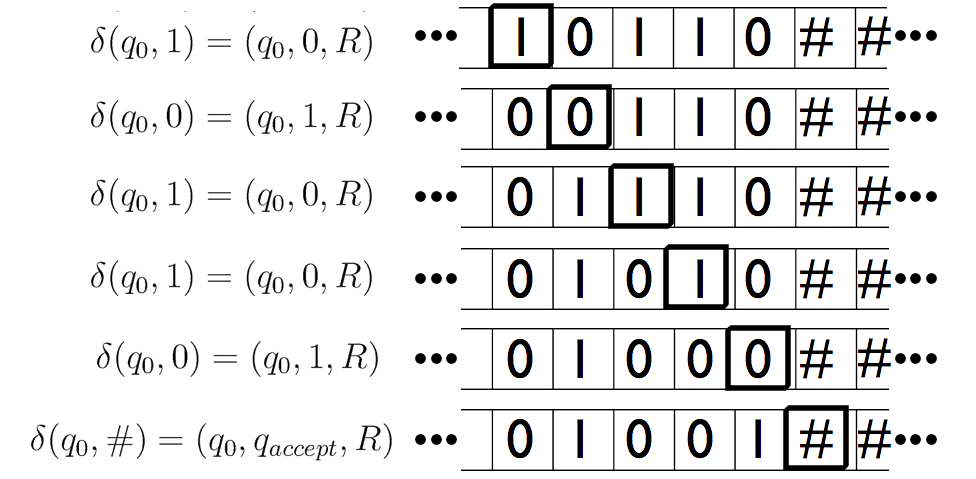
\includegraphics[width=6in]{turing-example}}
  \caption{Computation sequence for a simple Turing machine sequence.
    The darkly outlined squares represent the location of the tape
    head at each step.}
  \label{turing-example}
\end{figure}

Note that we can express all the information about the current state
of a machine $M$ as a 3-tuple, $(n, q, \gamma)$, where $n \in
\naturals$ represents the offset of the current position of the tape
head from the leftmost cell, $q \in Q$ is the current state of the
machine, and $\gamma \in \Gamma^*$ represents the string of symbols
on the tape, read in order from left to right, up to the point where
all subsequent symbols are blanks.  Such a tuple is called a
\textbf{configuration} of $M$. On an input, $w \in \Sigma^*$, $M$
begins in the initial configuration given by $(0, q_0, w)$ and
proceeds to compute as described above until it transitions into
$q_{accept}$ or $q_{reject}$, at which point the machine is said to
\textbf{halt} and output whatever string is written on its tape.
If, on input $w$, $M$ halts in state $q_{accept}$, we say that $M$
\textbf{accepts} $w$.  Similarly, we say that $M$ \textbf{rejects}
$w$ if it halts in state $q_{reject}.$ \\

An important feature of the Turing Machine model is the fact that
there is no guarantee a given machine will halt on a given input; a
machine may compute in such a way that it never reaches $q_{accept}$
or $q_{reject}$. The set of strings for which a machine $M$ does halt
is referred to as the \textbf{halting set} of $M$, which we denote
by $\halting_M$.\\

Since each step in the above procedure is deterministic, we can see
that a machine $M$ defines a partial function on the strings
defined by its input alphabet:
$$\mfunctype{f_M}{\Sigma^*}{\Gamma^*}$$

$$f_M(w) = \twopartdef{\textnormal{output of M on input w}}{w \in \halting_M}
{\textnormal{undefined}}{w \notin \halting_M}$$.
\newline

A machine $M$ also defines a total function on its halting set:

$$\mfunctype{\chi_M}{\halting_M}{\set{0,1}}$$

$$\chi_M(w) = \twopartdef{0}{\textnormal{M rejects w}}
{1}{\textnormal{M accepts w}}$$;

$\chi_M$ is sometimes referred to as the \textbf{characteristic} function of $M$.\\

\begin{definition}{\textbf{Turing-Computable Function}}\\

  A function \functype{g}{S}{T} is said to be
  \textbf{Turing-Computable}, or simply \textbf{computable} if there
  exists a Turing Machine $M$ such that
  
  $$\forall w \in S: f_M(w) = g(w)$$
  
\end{definition}

\setstretch{1.2}

\section{Decision Problems}

The Turing Machine provides us with a model for what it means
mathematically to perform a computation on a given input.  We now
want to consider what it means for a Turing Machine to ``solve''
some particular problem.  Our main idea here is that we can define a
problem as a language of strings, each of which corresponds to a
particular instance of the problem.  A Turing Machine ``solves'' a
problem if it accepts only those instances of a problem that share
some important property.

\begin{definition}{\textbf{Decision Problem}}\\
  
  A \textbf{decision problem} over an alphabet $\Sigma$ is a set of
  strings

  $$S \subseteq \Sigma^*$$,

  and a partition of $S$ into subsets $S_{yes}$ and $S_{no}$.\\
\end{definition}

A decision problem is said to be \textbf{recognizable} if there
exists a Turing Machine $M$ that accepts exactly $S_{yes}$ and no
other inputs. (Note that $M$ can either reject or fail to halt for
inputs in $S_{no}$.)  Such a machine $M$ is said to
\textbf{recognize} $S$.
\\

A decision problem is said to be \textbf{decidable} if there exists
a Turing Machine, $M$ that accepts exactly $S_{yes}$ and rejects all
other inputs. Such a machine $M$ is said to \textbf{decide} $S$.

\subsection*{Examples of Decision Problems}

\begin{enumerate}

\item \textbf{EVEN}\\
  $S = \mathbb{N}$\\
  $S_{yes} = \set{a \in S \mid \exists b \in \mathbb{N}$$\suchthat a = 2b}$

\item \textbf{SUBSET SUM}\\
  $S = (x_1, \ldots, x_n, T)$\\
  $S_{yes} = \set{s \in S \mid \exists X \subseteq \set{x_1, \ldots
      x_n} \suchthat \sum\limits_{x_i \in X}x_i = T}$

\item \textbf{HALTING}\\
  $S = \{\textnormal{encodings of Turing Machines}\}$\\
  $S_{yes} = \{$ encodings of Turing Machines that halt on all inputs $\}$
\end{enumerate}

\section{Time Complexity and the Class P}

For most practical purposes, it is not enough (or even particularly
interesting) to show that a problem is decidable, since decidability
tells us nothing about the resources necessary to solve a particular
problem.  One of the most important measures we have for
understanding the difficulty of solving a problem is its
\textbf{Time Complexity}, which we define in terms of the
relationship between the size of a problem instance and the number
of steps required for any Turing Machine to decide that instance.
\\

Let $size(w)$ denote the number of symbols in a string $w$.  A Turing
Machine $M$ is said to decide a language $S$ in time $O(g(n))$ (read
``big-oh $g(n)$'' or ``order $g(n)$'') if the following conditions
hold:

\begin{enumerate}
\item $M$ decides $S$
\item There exists a constant $c$ such that $\forall w \in S$, $M$ halts on
  input $w$ after at most $c \cdot g(size(w))$ computation steps.
\end{enumerate}

Note that if $f(n) < g(n)$, and some $M$
computes in $O(f(n))$ time, then $M$ also computes in $O(g(n))$
time.\\

Given this characterization of time complexity, an obvious question is
the following: which problems ``simple enough'' for us to compute. A
useful answer to this question has been the class $P$
(\textbf{P}olynomial Time), defined as the set of all problems which
can be solved in time
polynomial in input size. \\

\begin{definition}{\textbf{The Complexity Class P}}\\

  A problem $S$ is said to be a member of the \textbf{complexity
    class $P$} if there exists a Turing Machine $M$ and a constant
  $q$ such that $M$ decides $S$ in time $O(n^q)$.
\end{definition}

In general, a Turing Machine that always halts in $O(n^q)$ time for
some fixed $q$ is said to compute in \textbf{polynomial time}.

The class $P$ has a number of features which have made it attractive
as a model for problems which are computationally tractable.  From a
theoretical perspective, $P$ is convenient to work with because it
remains relatively robust against changes to one's model of
computation.  From a practical perspective, most of the interesting
problems in $P$ have been found to have algorithms that run in a
reasonable amount of time.  Though there are exceptions to this
observation (a problem which is solvable in $O(n^{1,000,000})$ time
may as well be unsolvable for most purposes), in practice we have
mostly found it to be the case that the problems in $P$ that we care
about can be solved efficiently.

\subsection*{Examples of Problems known to be in P}

\begin{enumerate}
\item{Shortest Path between Graph nodes (Solvable using
    breadth-first search in $O(n^2)$ time.}
\item{Greatest Common Divisor for Integers (Solvable via the Euclidean
    algorithm in $O(\log{n})$ time.)}
  
\item $n \times n$ Matrix Multiplication (Solvable via naive methods
  in $O(n^3)$ time.  Sub-matrix decomposition methods exist to
  compute in sub-cubic time.  For example, the Strassen algorithm
  runs in $O(n^{\log_2 7})$. \cite{S69}
    
\end{enumerate}

\section{The Class NP}

Another complexity class of theoretical and historical interest is
$NP$ (\textbf{N}ondeterministic \textbf{P}olynomial Time).  There
are several definitions of $NP$ which turn out to be equivalent, but
one important definition is its characterization in terms of
polynomial time verifiability.  Roughly speaking, a language $S$ is
verifiable by a Turing Machine $M$ if, for each $s$ in $S_{yes}$,
there is some extra piece of information, usually called a
\textbf{witness} or a \textbf{certificate} for $s$, which can be
used by $M$ to prove that $s \in S_{yes}$. $NP$ can be defined as
the class of problems for which there exist efficient (i.e.,
polynomial-time) verifiers. One way of intuitively understanding this
characterization of $NP$ is that it captures the class of problems
for which we can quickly check whether or not a candidate solution
is correct.

\begin{definition}{\textbf{Verifier}}\\

  A \textbf{verifier} for a language $S$ is a Turing Machine, $M$ such that:

  $$\forall s \in S, \text{ there exists a } w \suchthat M \text{ accepts } (w, s)$$ 

  and
  $$\forall s \notin S, \text{ there does not exist a } w \suchthat M \text{ accepts } (w, s)$$
  
\end{definition}
\begin{definition}{\textbf{The Complexity Class NP}}\\
  
  A problem $S$ is said to be a member of the class $NP$ if there
  exists a Turing Machine $M$ and constant $q$ such that:

  \begin{enumerate}
  \item $M$ is a verifier for $S$.
  \item $\forall s \in S$, M accepts $(w, s)$ in time $O(size(s)^q)$
  \end{enumerate}
  
\end{definition}

\subsection*{Examples of Problems in NP}

\begin{enumerate}
\item \textbf{SUBSET SUM} (See definition above)

  For each instance $s = (x_1, x_2, \ldots, x_n,
  T)$, a satisfying subset $X \subseteq \set{x_1, x_2, \ldots x_n}
  \suchthat$ $\sum\limits_{x_i \in X}x_i = T$ can serve as a witness
  if $s \in S_{yes}$.  If $s \in S_{no}$, then by definition no
  such witness exists.

\item \textbf{3-SAT}

  An instance of 3-SAT is a set of boolean variables, $\set{x_1,
    x_2, \ldots x_n}$ and a set $\set{\phi_1, \phi_2, \ldots
    \phi_m}$ of boolean formulae of the form $(\tilde{x}_i \vee \tilde{x}_j \vee
  \tilde{x}_k)$, where $\tilde{x}_i$ is either $x_i$ or $\bar x_i$.  An instance
  is a yes-instance if there exists an assignment of $\set{True, False}$
  to the variables $\set{x_i}$ such that all the $\phi_J$ evaluate to 
  $True$.\\

  If an instance, $S$ of \textbf{3-SAT} is a yes-instance, then we
  can verify this fact using a satisfying assignment as a witness
  by simply checking that all the $\phi$ are satisfied under that
  assignment.  Again, if $S$ is a no-instance, then by definition
  no such witness can exist.

\end{enumerate}

\section{Polynomial-Time Reductions and NP-Completeness}

An important technique in analyzing the complexity of problems is
showing that a given problem $A$ is, in a sense, ``no harder
than'' some other problem $B$.  We do this by showing that we can,
in polynomial time, convert any instance of $A$ into an instance
$B$ in such a way that we always map elements of $A_{yes}$ to
elements of $B_{yes}$ and elements of $A_{no}$ to elements of
$B_{no}$.  

\begin{definition}{\textbf{Polynomial-Time Reduction}}
  
  A Language A is \textbf{polynomial time reducible} to language
  B, written $A \leq_P B$, if there exists a polynomial-time
  computable function, f, such that: 
  $$\forall w \in A \mid f(w) \in B_{yes} \Leftrightarrow w \in A_{yes}$$
  
\end{definition}

Since polynomials are closed under addition, we can see
immediately that if $A \leq_P B$ and $B \in P$, then $A \in P$ as
well, since we can decide any instance of $A$ in polynomial time
by first converting it into an instance of $B$, which we can then
decide in polynomial time to return the appropriate result.  The
same argument shows that if $A \leq_P B$ and $B \in NP$, then $A \in
NP$.\\

Perhaps one of the most surprising results in complexity theory was
the independent discovery by Stephen Cook and Leonid Levin of NP
problems which are ``as hard as'' any other problems in NP. \cite{C71}

\begin{definition}{\textbf{NP-Hard and NP-Complete}}\\

  A problem $S$ is said to be \textbf{NP-Hard} if every problem in
  $NP$ is polynomial time reducible to $S$.\\
  
  A problem $S$ is said to be \textbf{NP-Complete} if it is
  NP-Hard and in NP.\\
\end{definition}

An immediate consequence of the above definition is the following:

\begin{proposition}{If $S$ is NP-Complete, and $S' \in NP$, then
    $S \leq_P S' \textnormal{implies that}$ $S'$ is NP-Complete.}
\end{proposition}
\begin{proof}
  Since we are given that $S' \in NP$, all that we need to show is
  that $S'$ is NP-Hard.  Let $T$ be a problem in NP.  Since $S$ is
  NP-Complete, there exists a polynomial-time computable function
  \functype{f}{T}{S} such that $f(t) \in S_{yes} \Leftrightarrow t
  \in T_{yes}$. Since $S \leq_P S'$, there exists a
  polynomial-time computable function, \functype{g}{S}{S'} such
  that $f(s) \in S'_{yes} \Leftrightarrow s \in S_{yes}$.  Then
  the function $f \circ g$ is a polynomial time function from $T
  \rightarrow S'$ such that $(f \circ g)(t) \in S'_{yes}
  \Leftrightarrow t \in T_{yes}$.  So we have that $T \leq S'$,
  which implies that $S'$ is NP-Hard.
\end{proof}\\

The above proposition gives us a means of using known NP-Complete
problems to show that other problems are also NP-Complete.  This is
the usual way that one goes about showing that a given problem is
NP-Complete.  Of course, this method does us no good if we don't have
any NP-Complete problems to reduce from!  The following theorem
provides us with an initial problem to reduce from.  The interested
reader may refer to \cite{S06} or \cite{C71} for details.

\begin{theorem}{Cook-Levin Theorem (1971)}: 3-SAT is NP-Complete
\end{theorem}
\begin{proofsketch}
  The main idea of the proof is that one can take an instance of any
  NP problem and use it to encode sequences of Turing Machine
  configurations in boolean formulae in such a way that the formulae
  are satisfiable if and only if the configurations correspond to an
  accepting computation for some verifier of the problem instance.
\end{proofsketch}

\section{Binary Integer Programming Feasibility is NP-Complete}

We are finally in a position to give a demonstration of the fact
that the task of determining whether a Binary Integer Programming
problem has a feasible solution is NP-Complete. We do so via a
reduction from \textbf{3-SAT}.

\begin{theorem}
  Binary Integer Programming Feasibility is NP-Complete.
\end{theorem}

\begin{proof}

  Let $s = (\set{x_1, x_2, \ldots x_n}, \set{\phi_1, \phi_2, \ldots
    \phi_m})$ be an instance of 3-SAT.  We can construct a Binary
  Integer Program which is feasible if and only if $s$ has a satisfying
  assignment as follows:

\begin{enumerate}
\item For each $x_i$ in the description of s, add variables $x_i,
  \bar{x_i}$ to our program.
\item For each pair ($x_i, \bar{x_i}$), add the constraint that $x_i + \bar{x_i} = 1$
\item For each clause $\phi = (\tilde{x}_i, \tilde{x}_j,
  \tilde{x}_k)$, add to our program the constraint that $\tilde{x}_i +
  \tilde{x}_j + \tilde{x}_k \geq 1$
\end{enumerate}

It is clear that there is a satisfying assignment to the original
\textbf{3-SAT} instance if and only if there is a feasible solution to
our constructed binary integer program.  Moreover, since our
construction only requires that we perform a constant number of
operations for each variable and each clause in the \textbf{3-SAT}
instance, it is clear that we can compute our reduction in polynomial
time.  Thus we have that \textbf{3-SAT} $\leq_P$ \textbf{BIP-FEAS}.
All that remains for us to show is that \textbf{BIP-FEAS} is in NP.
But this is also trivial, since we can easily verify whether a
candidate solution meets all the program constraints by simply
plugging in the values for each variable, which requires at most
linearly many operations in the number of constraints.
\end{proof}

\newpage 
\section*{References}

\beginrefs

\bibentry{B98}{\sc Blum et al.},
``Complexity and Real Computation,''
{\it Springer-Verlag New York, Inc.}
New York City, 1998

\bibentry{C71}{\sc Cook, Steven}, ``The complexity of theorem-proving
procedures,'' {\it Proceedings of the Third Annual ACM Symposium on
  Theory of Computing. pp. 151 - 158.}  ACM New York, 1971.

\bibentry{M60}{\sc McCarthy, John},
``Recursive Functions of Symbolic Expressions
and Their Computation by Machine, Part I,''
{\it Communications of the ACM, April 1960.}

\bibentry{S06}{\sc Sipser, Michael},
``Introduction to the Theory of Computation,''
{\it Course Technology.}
Boston MA, 2006

\bibentry{S69}{\sc Strassen, Volker}, ``Gaussian Elimination is not
Optimal,'' {\it Numer. Math. Volume 13. pp 354-356} 1969
\endrefs

\end{document}